% !TeX spellcheck = cs_CZ
\wikitextrule
\begin{example}\label{mai:exam035}
  \textbf{Fyzika — Ohmův zákon:}\newline\small
  Z elektřiny víme, že některé vodiče či elektrické prvky se při průchodu elektrického proudu 
  chovají podle zákona linearity: Proud, který jimi protéká, závisí přímo úměrně na přiloženém 
  napětí (obr. \ref{mai:fig036}). Platí \(I(U) = R^{-1 }U\) s konstantou úměrnosti \(R^{-1}\), kde 
  \(R\) je elektrický odpor vodiče (prvku).

  Pozn. 1: Předpokládáme, že elektrický odpor voltmetru je tak velký, že proud jím procházející je 
  z hlediska přesnosti měření zanedbatelný.
  
  Pozn. 2: Graf závislosti proudu na napětí na obrázku \ref{mai:fig036} může pro vyšší hodnoty 
  napětí vykazovat odchylku od linearity (přímkové závislosti), neboť se prvek při vyšším proudu 
  zahřívá a jeho odpor roste.
  
  {\centering
    \captionsetup{type=figure}
    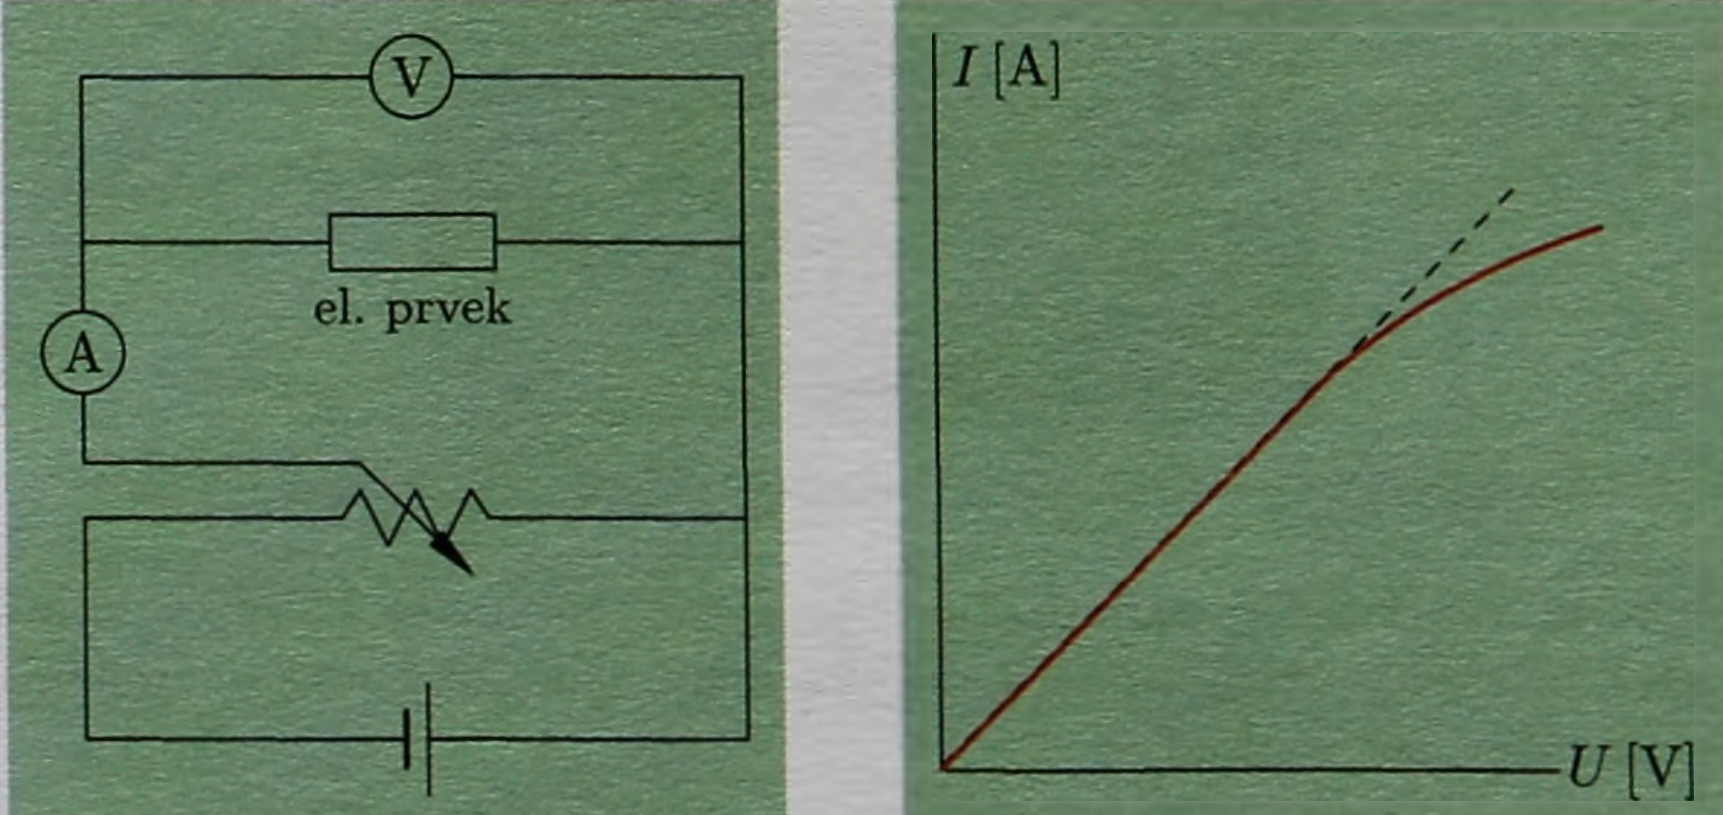
\includegraphics[width=0.4\linewidth]{mai_fig036.png}
    \captionof{figure}{Chování lineárního vodiče (Ohmův zákon). \cite[s.~15]{Musilova2009MA1}}
    \label{mai:fig036}
    \par}  
  \normalsize
\end{example}